\subsection{Implementation}
The sequential discriminant implementation is inplemented in the
\texttt{SequentialEstimation} class (see Section \ref{sec:seq_est}). The
class comprises of 3 main functions to generate the discriminants along with 4
helper functions that classify points based on the discriminants, generate a
confusion matrix for the classifier, and plot the discriminants and the class
boundaries.

Discriminant calculations in \texttt{SequentialEstimation} make use of the
\texttt{ParametricClass} and \texttt{NonParametricClass} classes from Lab 1.
Each linear discriminant is represented by a MED boundary between the two
reference points. This is used to calculate the confusion matricies to identify
acceptable classifiers as well as in plotting and classifying points after the
overall sequential classifier is formed.

\subsection{Results}
%Images

% 4.2
When testing the classifier against the training data, the probability of error
will be zero. As opposed to parametric classifiers where the boundaries are generated from
the statistics of the sample, sequential discriminants form their boundaries by
ensuring that they capture each data point from the training set inside the
classifier. Thus, the training data will fall entirely into the correct
classifiers and the probability of error is zero.

% 4.3
\begin{table}
\centering
\caption{Error rates (\%) in classifying the test data}
\label{tab:error_rates}
\begin{tabular}{lrrrr}
\toprule
$J$ & min & $\mu$ & max & $\sigma$\\
\midrule
1 & 22.25 & 28.1375 & 35.25 & 3.3936\\
2 & 5.5 & 11.6375 & 21 & 4.3728\\
3 & 2.5 & 7.4625 & 18.25 & 4.5337\\
4 & 0.25 & 6.725 & 38.75 & 10.1472\\
5 & 0 & 10.1625 & 37 & 12.1421\\
\bottomrule
\end{tabular}
\end{table}

This result changes if the number of discriminants allowed is limited. Figure
\ref{fig:error_rates} shows how error rates generally decrease in inverse
proportion to the number of classifiers. It also shows, however, that while the
general trend is decreasing error, it is prone to random spikes due to the
nature of the classifier selection.

\begin{figure}
\label{fig:error_rates}
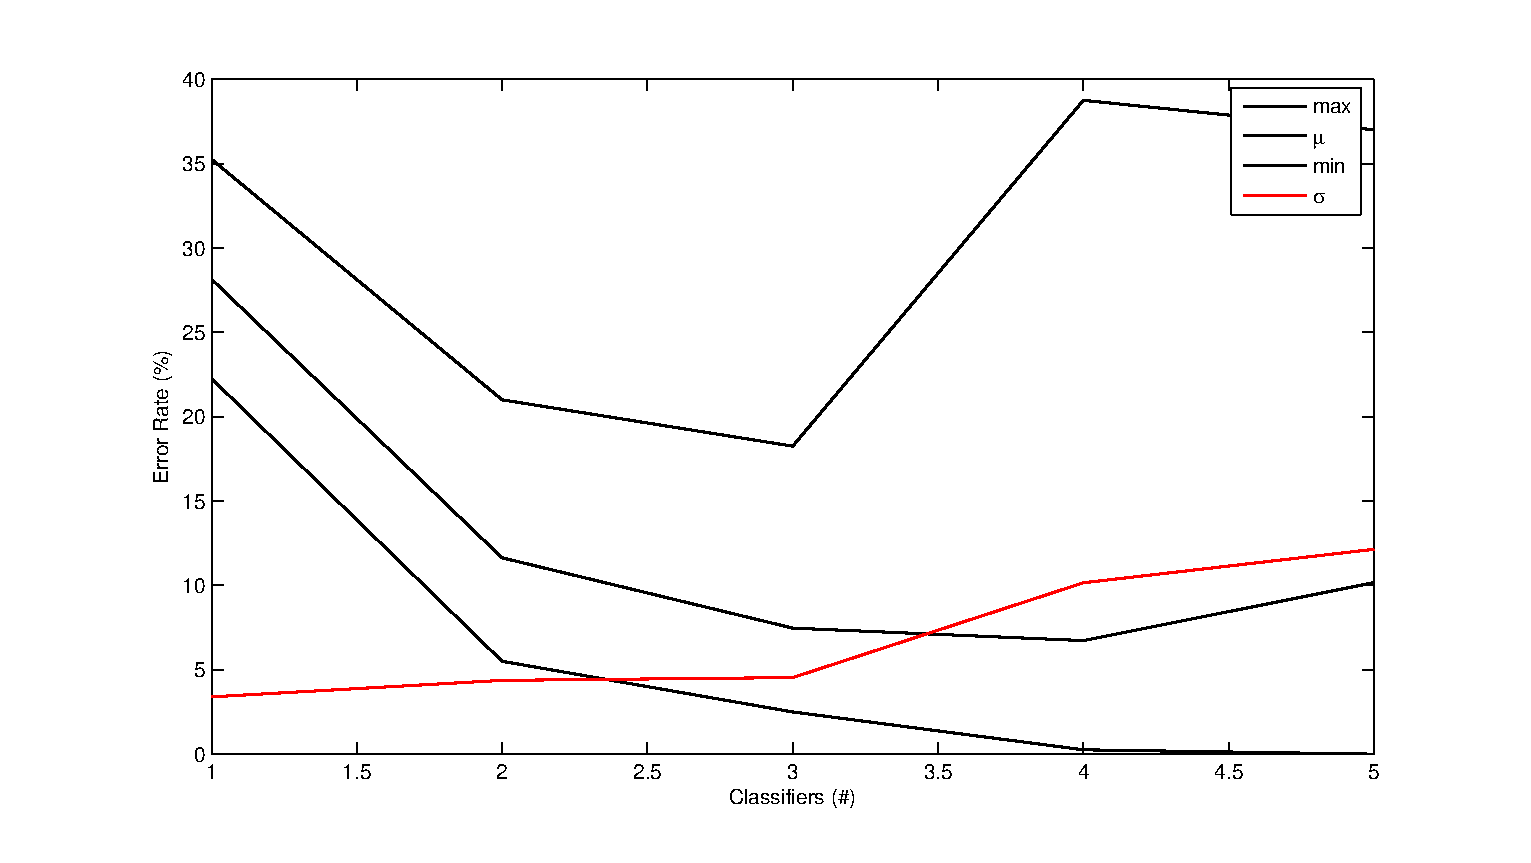
\includegraphics[scale=0.6]{sequence_error_plots}
\caption{Plot of error rates for different numbers of discriminants.}
\end{figure}

Limiting the number of point pairs to test would also shift the results
somewhat. The shift would depend on how the new classifiers were selected. One
possible method would be to track how many points from each class fall on the
correct side of a potential classifier and select the one with the highest
number or proportion of correct points in a class after a specified number of
iterations. This method would likely smooth class shapes somewhat as some
outlier points may be neglected in a given sectioning.

Another strategy may be to simply stop after a number of iterations if a
suitable classifier has not been found. This could produce a rather random set
of classifiers, potentially cutting off large sections of a class in the
process.